\section{Исследование LQR}
Рассмотрим систему: 
\begin{equation}
    \dot{x} = Ax + Bu, \quad x_0 = \begin{bmatrix}1 & 1 & 1\end{bmatrix}^T
\end{equation}
где 
\begin{equation}
    \begin{array}{cc}
        A = \begin{bmatrix}
            8 & 1 & 11 \\ 
            4 & 0 & 4 \\
            -4 & -3 & -7
        \end{bmatrix}, &
        B = \begin{bmatrix}
            -1 \\ -3 \\ 3
        \end{bmatrix}
    \end{array}
\end{equation}
\subsection{Управляемость собственных чисел}

Для определения управляемости собственных чисел рассмотрим вещественную Жорданову форму системы: 
\begin{equation}
    \dot{\hat{x}} = P^{-1}AP\hat{x} + P^{-1}Bu
\end{equation}
Где $P$ -- матрица собственных векторов матрицы $A$, а $\hat{x} = P^{-1}x$.
\begin{equation}
    A_j = \begin{bmatrix}
        -3  & 0  & 0 \\ 
        0  & 2  & -2 \\ 
        0  & 2  & 2 \\ 
    \end{bmatrix}\quad
    P = \begin{bmatrix}
        -1  & -2.12  & 0.71 \\ 
        0  & -1.41  & 0 \\ 
        1  & 1.41  & 0 \\ 
    \end{bmatrix}\quad 
    B_j = \begin{bmatrix}
        0 \\ 
        2.12 \\ 
        4.95 \\ 
    \end{bmatrix}
\end{equation}

Таким образом, последнее собственное число $\lambda_3 = -3$ не является управляемым. Соответственно, система не является полностью управляемой. 
Но, так как данное собственное число располагается в левой полуплоскости, то есть является устойчивым, то система является стабилизируемой. 

\subsection{Синтез регулятора}
Зададимся четырьмя матрицами весов $Q$ и $R$ для синтеза регулятора LQR: 
\begin{equation}
    Q_1 = \begin{bmatrix}
        2 & 0 & 0 \\ 
        0 & 2 & 0 \\ 
        0 & 0 & 2
    \end{bmatrix}, \quad
    R_1 = \begin{bmatrix}
        2
    \end{bmatrix}
\end{equation}
\begin{equation}
    Q_2 = \begin{bmatrix}
        2 & 0 & 0 \\ 
        0 & 2 & 0 \\ 
        0 & 0 & 2
    \end{bmatrix}, \quad
    R_2 = \begin{bmatrix}
        20
    \end{bmatrix}
\end{equation}
\begin{equation}
    Q_3 = \begin{bmatrix}
        20 & 0 & 0 \\ 
        0 & 20 & 0 \\ 
        0 & 0 & 20
    \end{bmatrix}, \quad
    R_3 = \begin{bmatrix}
        2
    \end{bmatrix}
\end{equation}
\begin{equation}
    Q_4 = \begin{bmatrix}
        20 & 0 & 0 \\ 
        0 & 20 & 0 \\ 
        0 & 0 & 20
    \end{bmatrix}, \quad
    R_4 = \begin{bmatrix}
        20
    \end{bmatrix}
\end{equation}
Таким образом, получаем пары матриц весов $Q_i$ и $R_i$, каждая из которых соответствует определенному критерию оптимальности. 
Будем называть матрицу $Q_i$ матрицей, отвечающий за штраф за отклонение состояния системы от желаемого значения, а 
матрицу $R_i$ -- матрицей, отвечающей за штраф за использование \textit{резкого} управления. 

На основе этих матриц будем синтезировать регулятор, минимизирующий функционал качества:
\begin{equation}
    J = \int_0^\infty \left( x^TQx + u^TRu \right) dt
\end{equation}
Для получения регулятор решим матричное уравнение Риккати при $v = 1$ для каждой пары матриц весов $Q_i$ и $R_i$:
\begin{equation}
    \begin{cases}
        A^T + PA + Q - vPBR^{-1}B^TP = 0 \\ 
        K = -R^{-1}B^TP
    \end{cases}
\end{equation}
Единственное решение данного уравнения будет существовать при том, что пара $(A, B)$ является стабилизируемой, пара $(Q, A)$ -- наблюдаемой, 
а матрица $R$ -- положительно определенной и матрица $Q$ -- положительно полуопределенной.

При этом соответствующее минимизированное значения функционала качества $J_min$ можно найти по формуле:
\begin{equation}
    J_{min} = x_0^TPx_0 
\end{equation}

Синтезируем регуляторы для каждой пары матриц весов $Q_i$ и $R_i$, получим следующие результаты:
\begin{equation}
    \begin{array}{cc}
        K_1 = \begin{bmatrix}
        -6.40  & 0.79  & -5.96 \\ 
        \end{bmatrix} & 
        J_1 = 30.903426 \\ 
        K_2 = \begin{bmatrix}
        -14.44  & 0.40  & -12.68 \\ 
        \end{bmatrix} &
        J_2 = 130.971703 \\
        K_3 = \begin{bmatrix}
        -3.64  & 0.85  & -3.55 \\ 
        \end{bmatrix} &
        J_3 = 121.680719 \\ 
        K_4 = \begin{bmatrix}
        -6.40  & 0.79  & -5.96 \\ 
        \end{bmatrix} &
        J_4 = 309.034256 \\ 
    \end{array}
\end{equation}

\subsection{Моделирование}
Проведем моделирование системы с регуляторами $K_i$ и начальными условиями $x(0) = \begin{bmatrix} 1 & 1 & 1 \end{bmatrix}^T$. 
Схема моделирования представлена на рисунке \ref{fig:scheme_lqr}, схема для вычисления функционала качества представлена на рисунке \ref{fig:scheme_lqr_j}.
\begin{figure}[ht!]
    \centering
    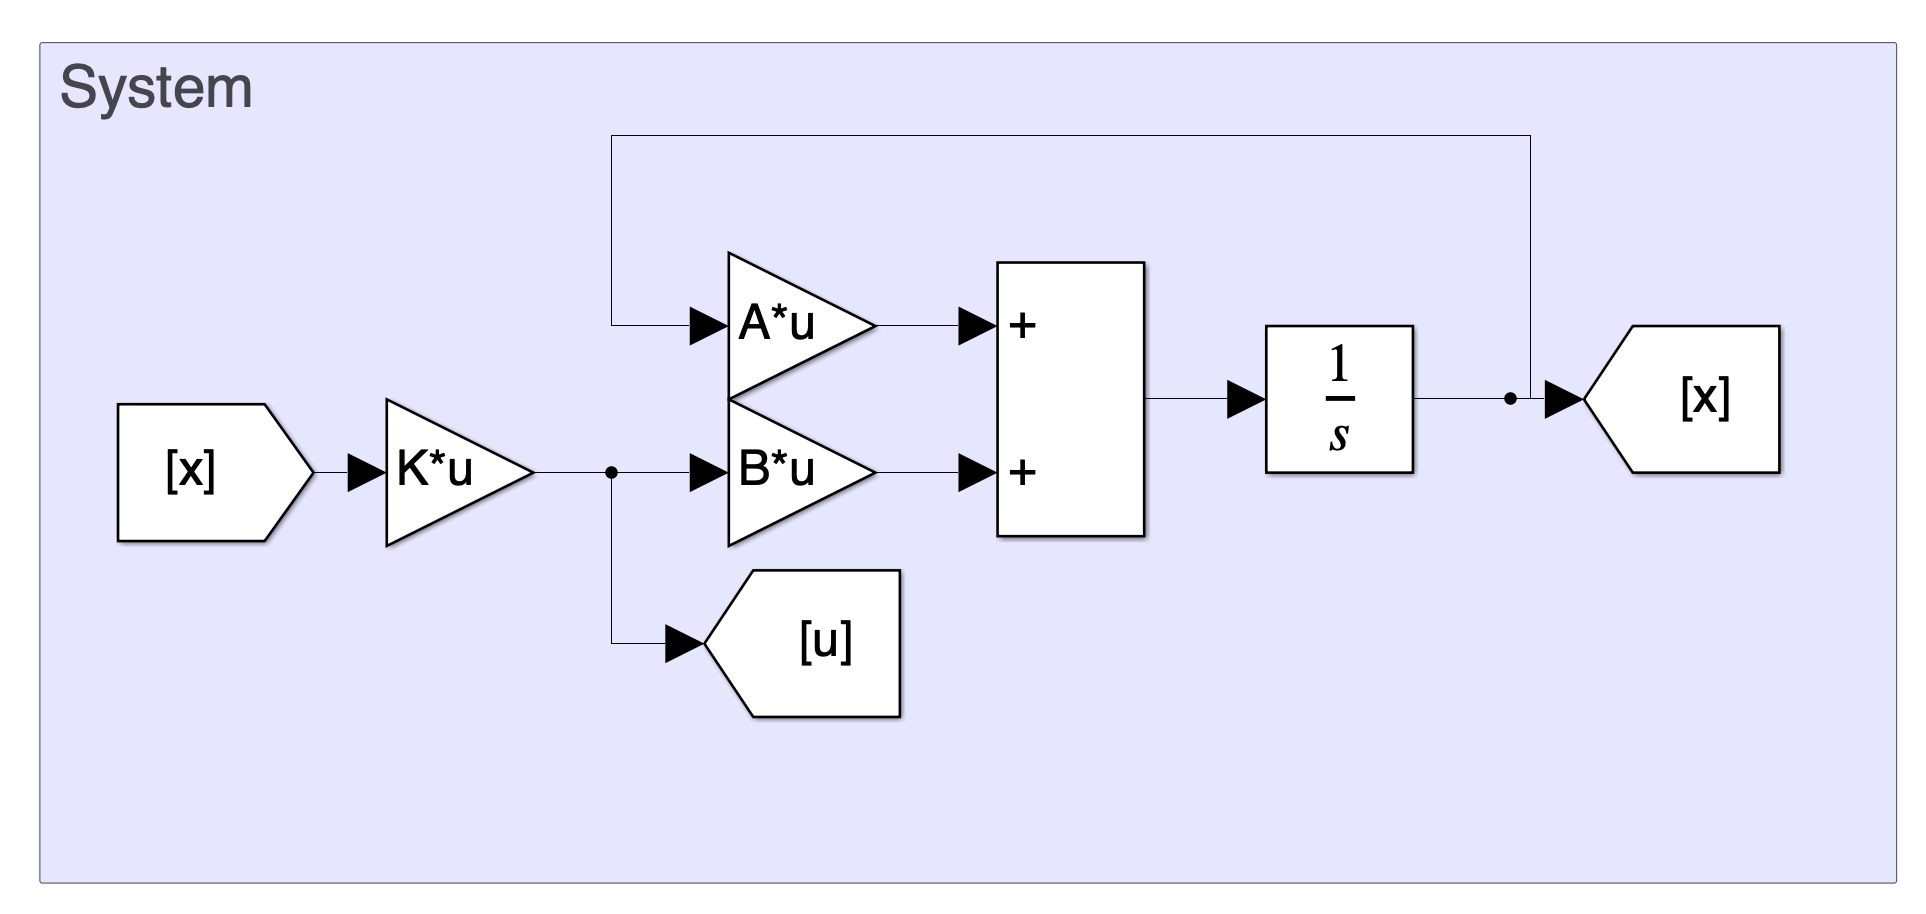
\includegraphics[width=0.8\textwidth]{media/task1_system_scheme.png}
    \caption{Схема моделирования системы с регулятором LQR}
    \label{fig:scheme_lqr}
\end{figure}
\begin{figure}[ht!]
    \centering
    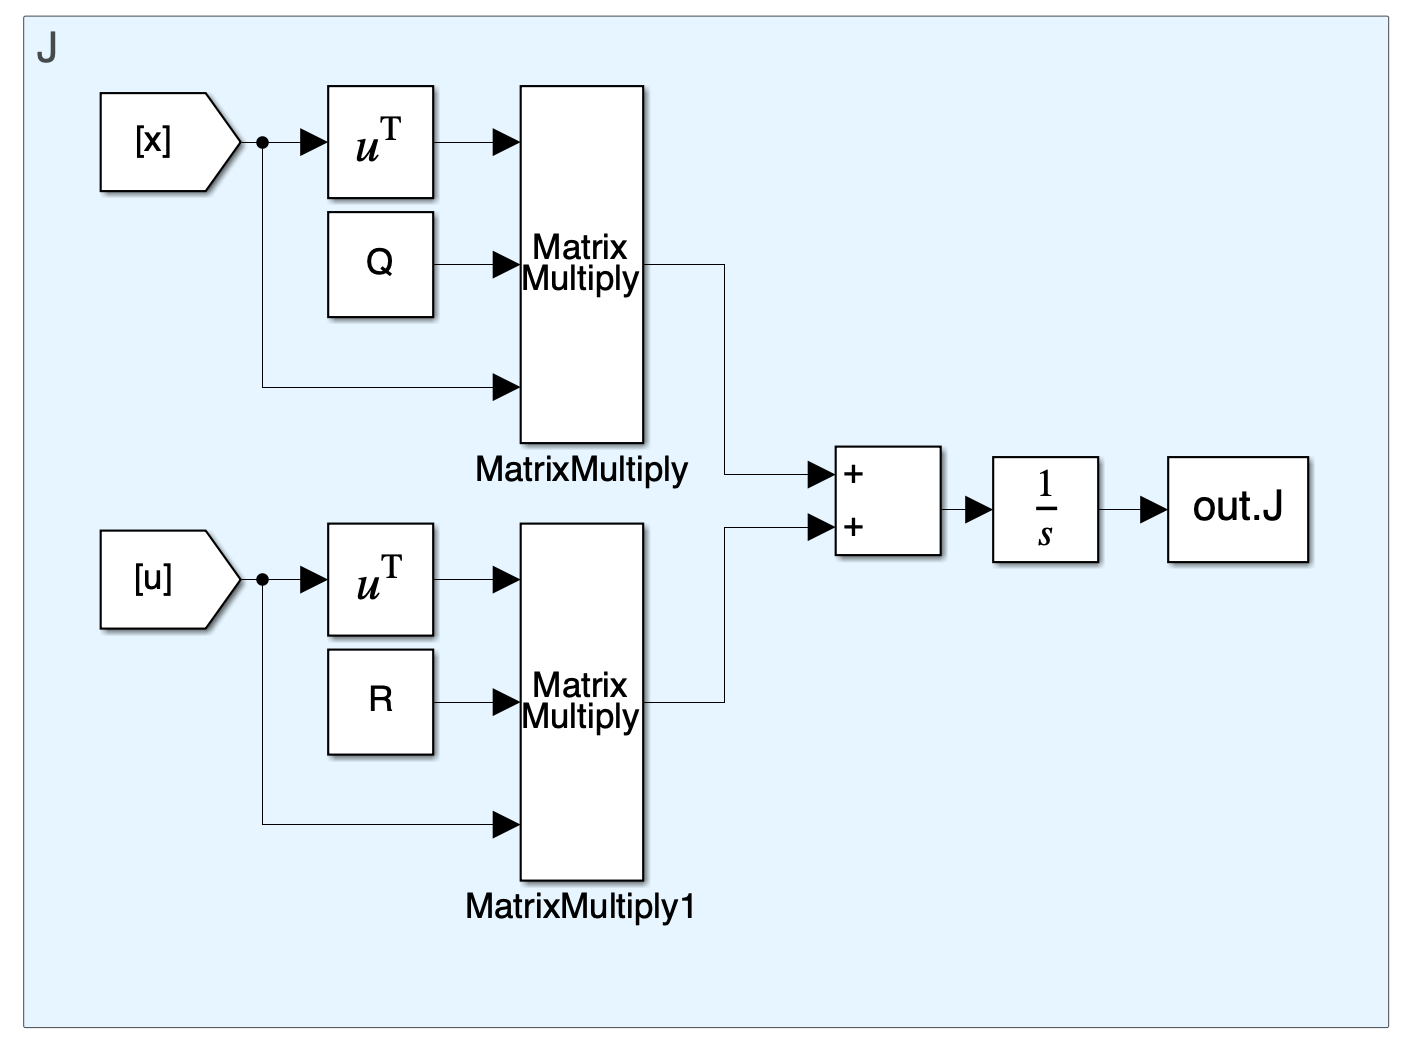
\includegraphics[width=0.8\textwidth]{media/task1_J_scheme.png}
    \caption{Схема вычисления функционала качества LQR}
    \label{fig:scheme_lqr_j}
\end{figure}

Результаты моделирования представлены на рисунках \ref{fig:task1_x_1} -- \ref{fig:task1_x_4} (состояние системы),
\ref{fig:task1_u} (сравнительный график управления для всех регуляторов), \ref{fig:task1_j} (сравнительный график функционала качества для всех регуляторов) и 
графиках \ref{fig:task1_x1_cmp_1} -- \ref{fig:task1_x3_cmp_1} (сравнительные графики состояния системы для регуляторов $K_i$).

\begin{figure}[ht!]
    \centering
    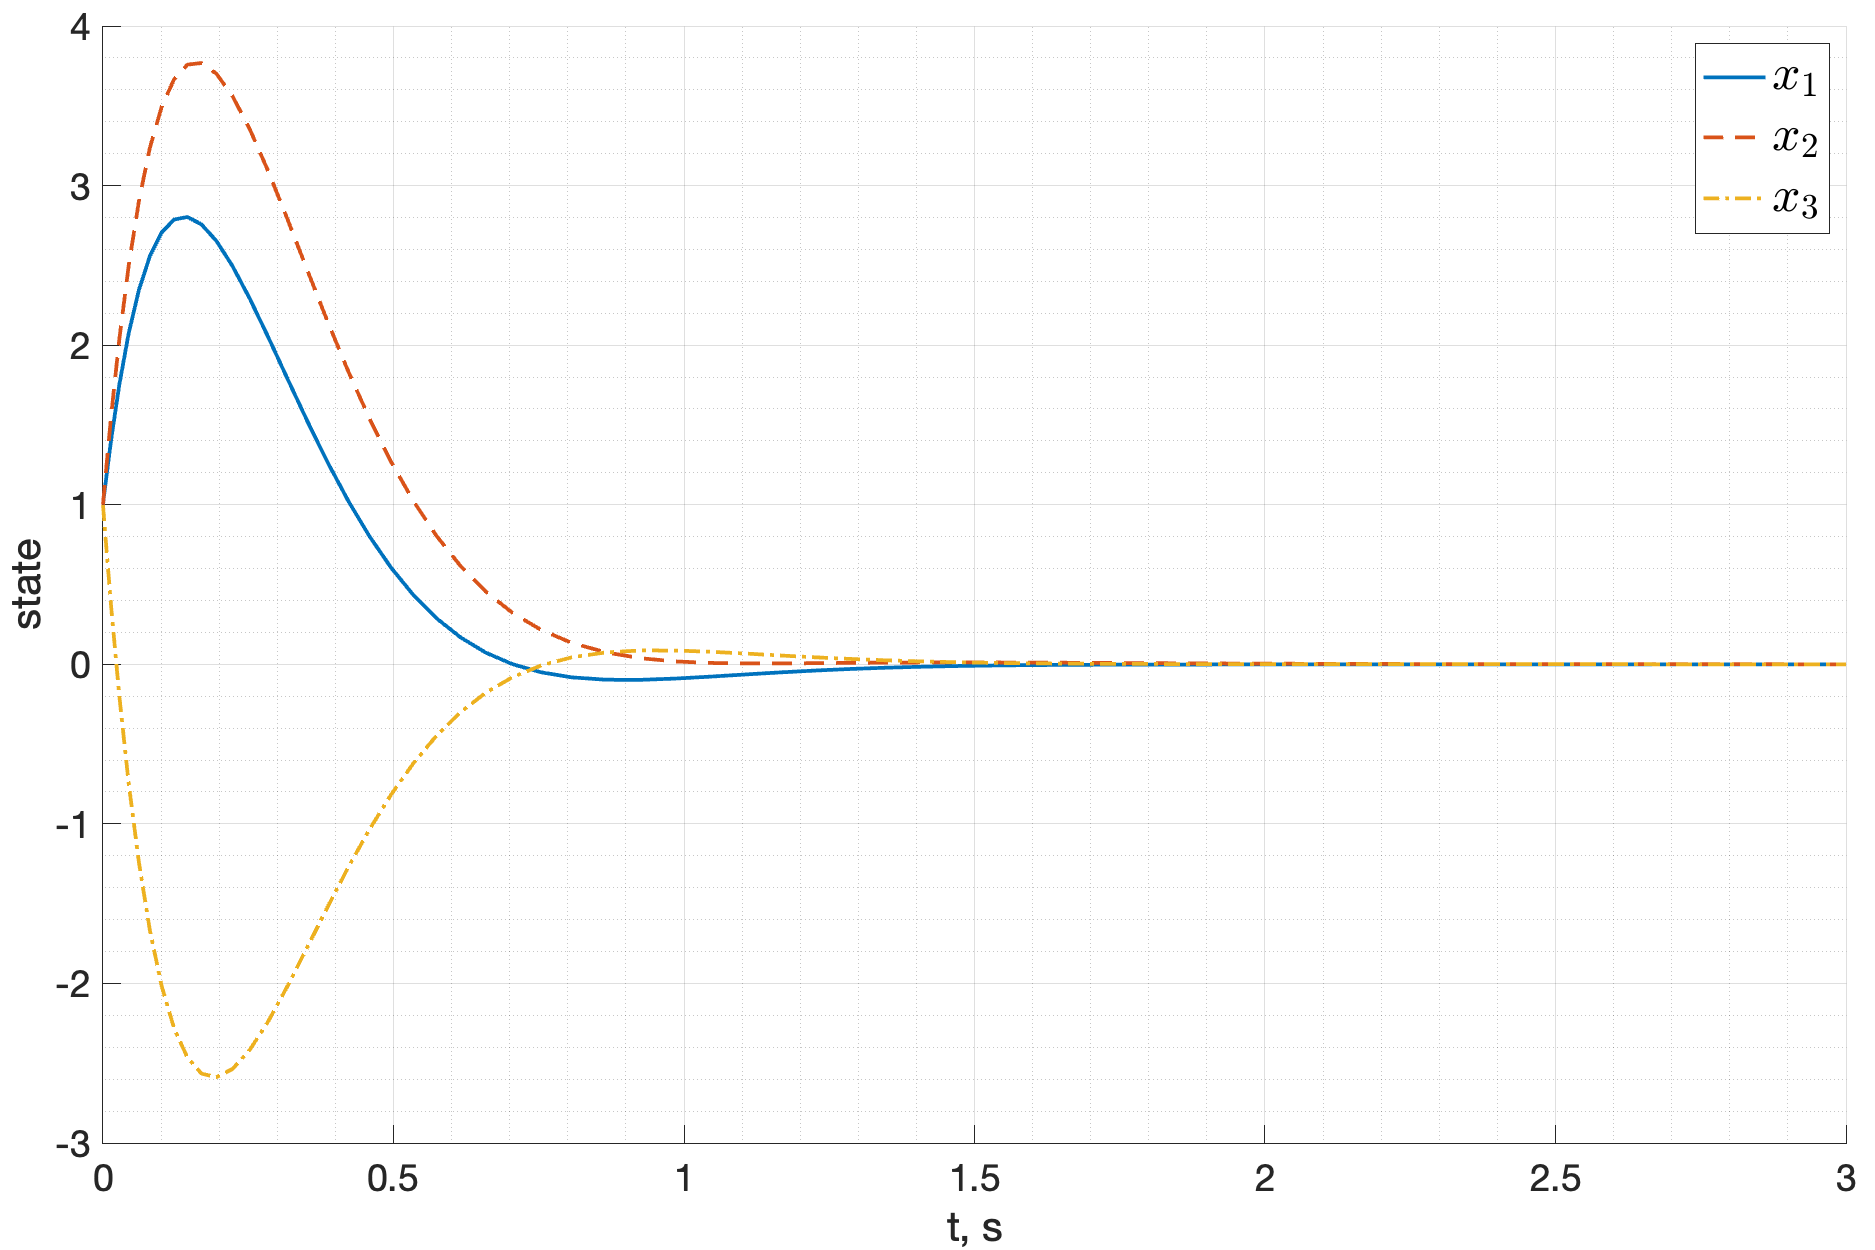
\includegraphics[width=\textwidth]{media/plots/lqr_task1/state_1.png}
    \caption{Состояние системы с регулятором $K_1$}
    \label{fig:task1_x_1}
\end{figure}
\begin{figure}[ht!]
    \centering
    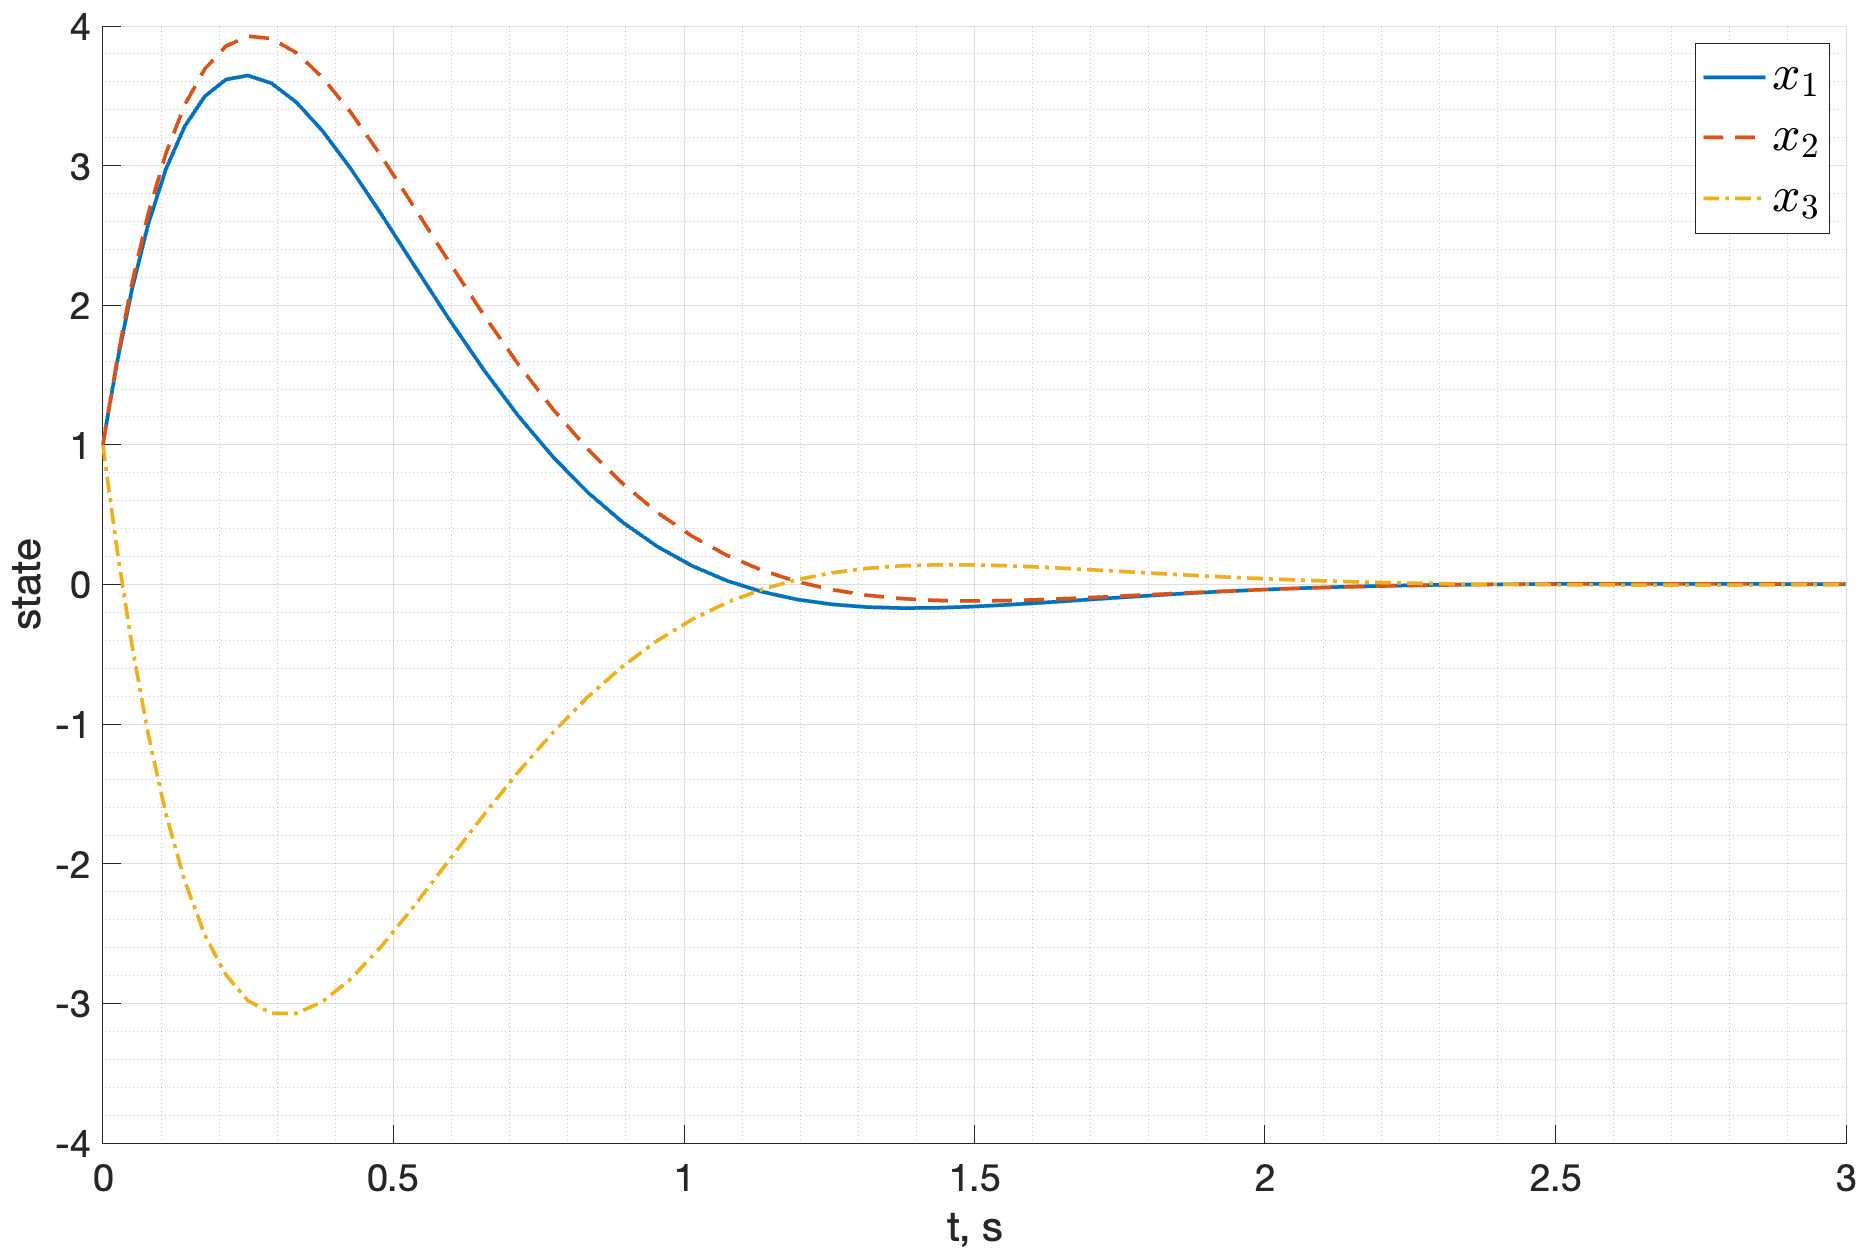
\includegraphics[width=\textwidth]{media/plots/lqr_task1/state_2.png}
    \caption{Состояние системы с регулятором $K_2$}
    \label{fig:task1_x_2}
\end{figure}
\begin{figure}[ht!]
    \centering
    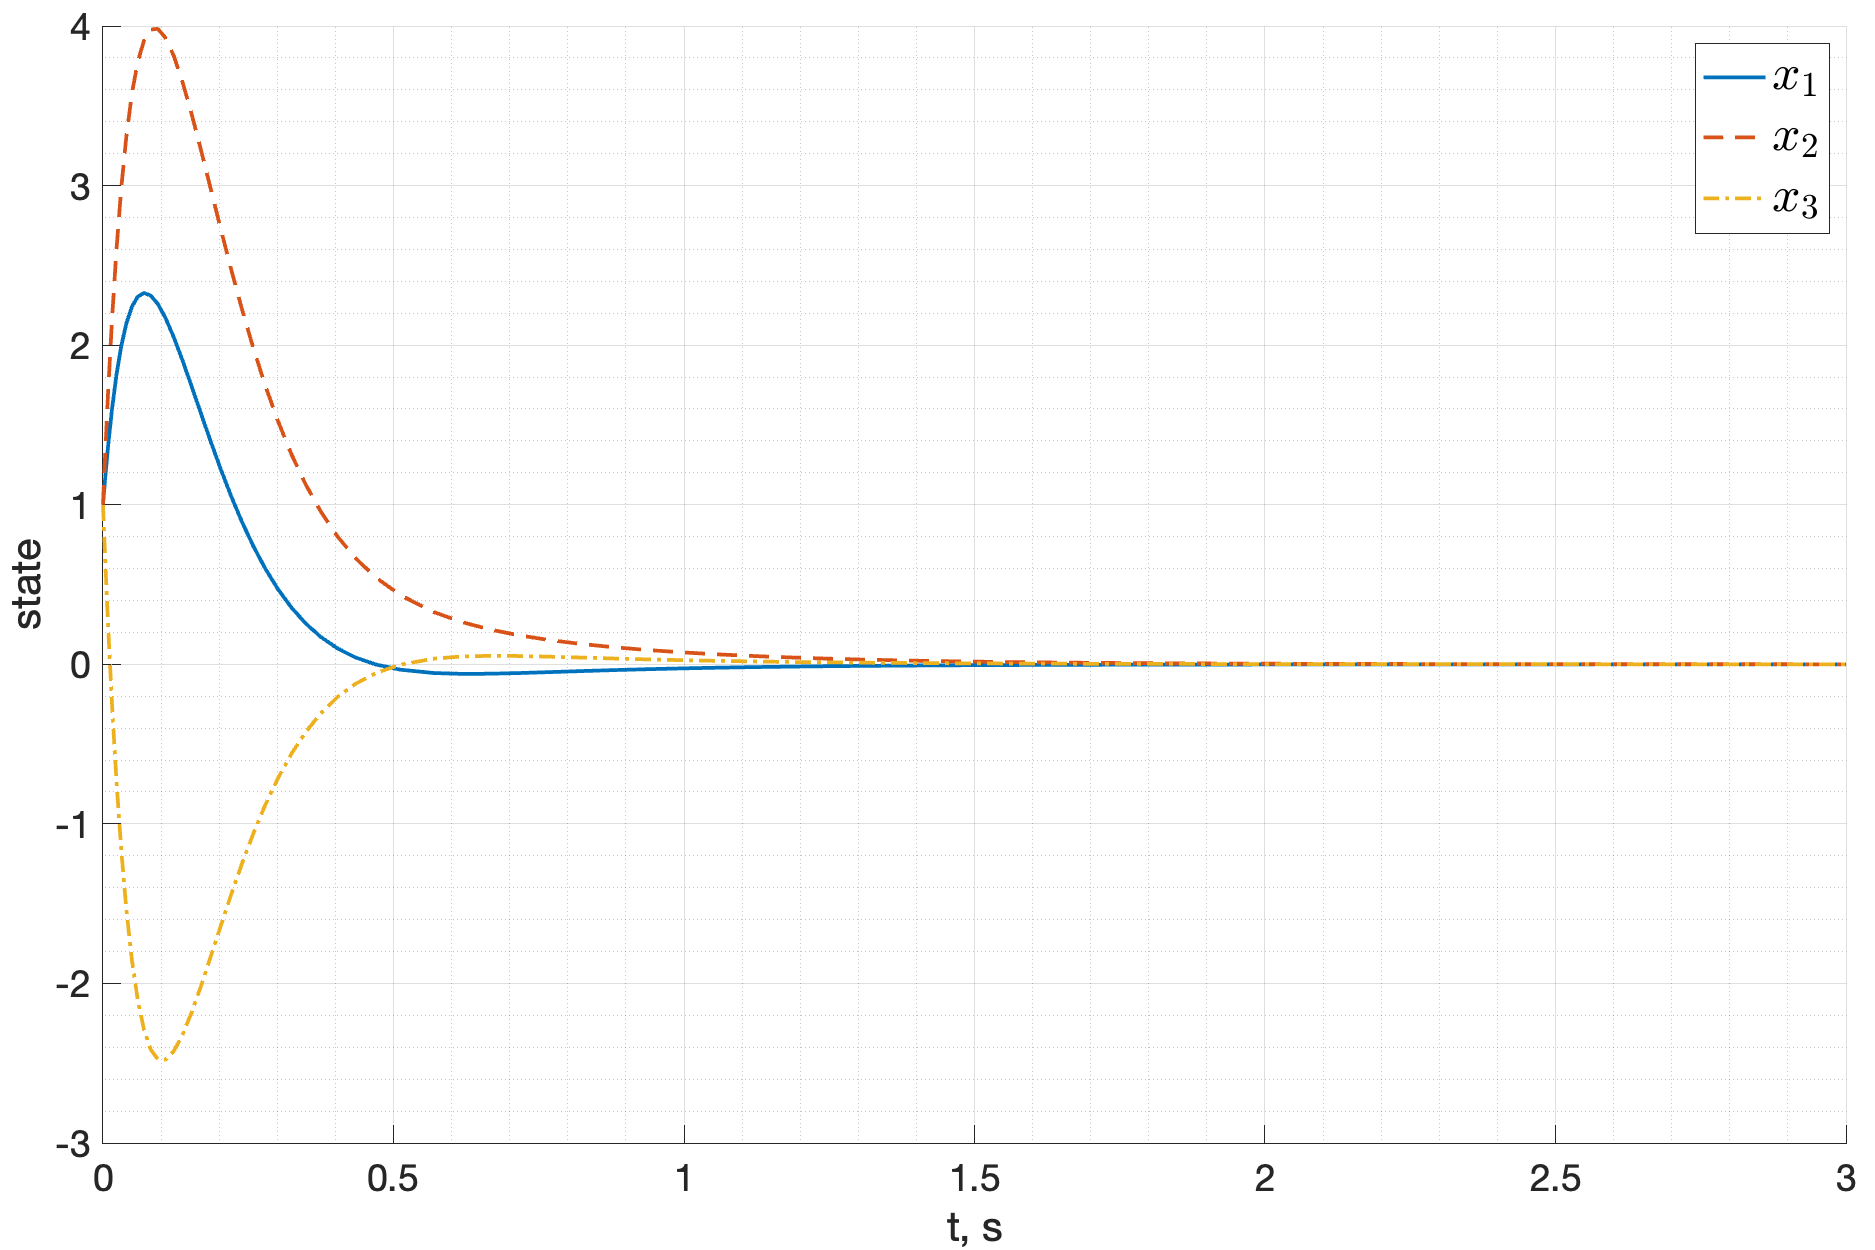
\includegraphics[width=\textwidth]{media/plots/lqr_task1/state_3.png}
    \caption{Состояние системы с регулятором $K_3$}
    \label{fig:task1_x_3}
\end{figure}    
\begin{figure}[ht!]
    \centering
    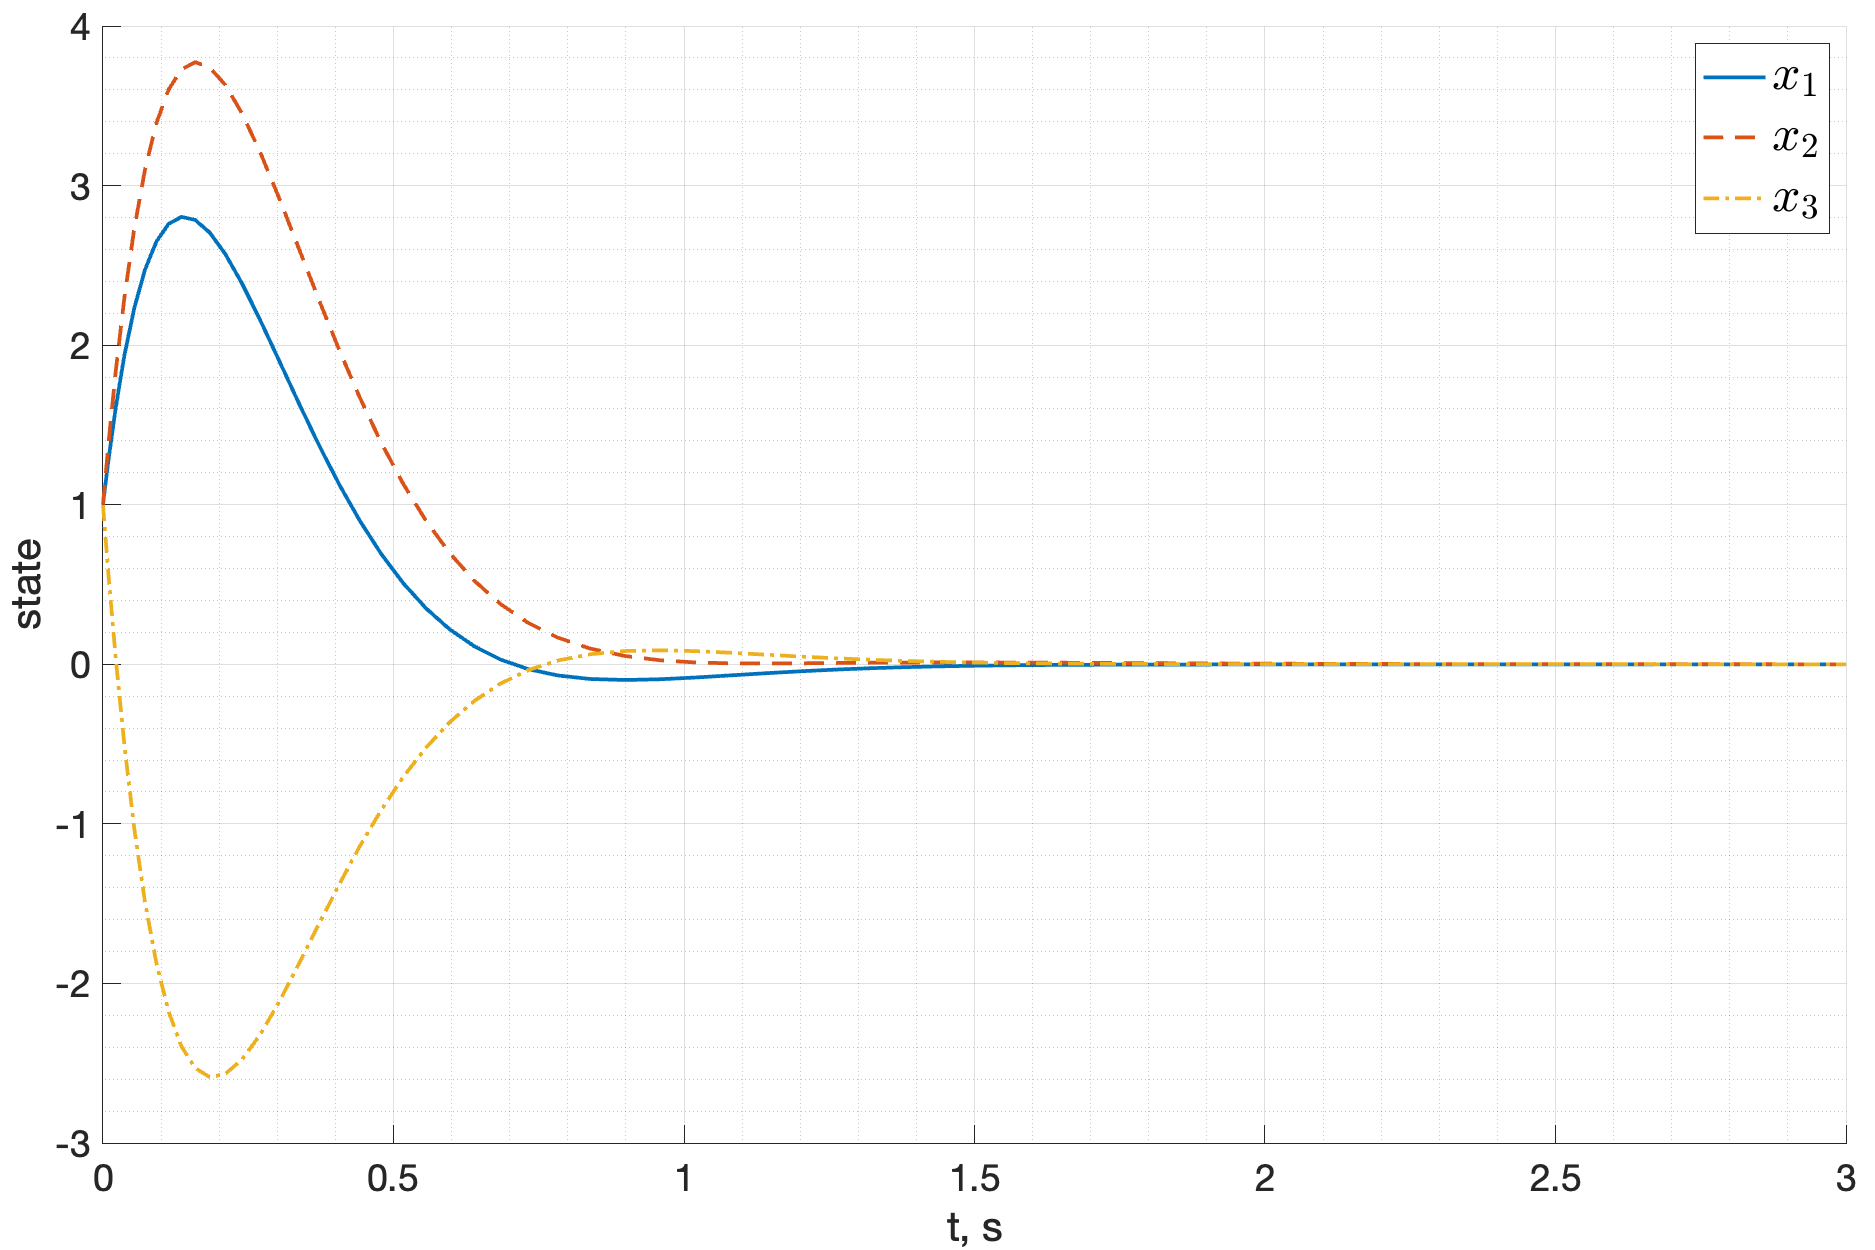
\includegraphics[width=\textwidth]{media/plots/lqr_task1/state_4.png}
    \caption{Состояние системы с регулятором $K_4$}
    \label{fig:task1_x_4}
\end{figure}
\begin{figure}[ht!]
    \centering
    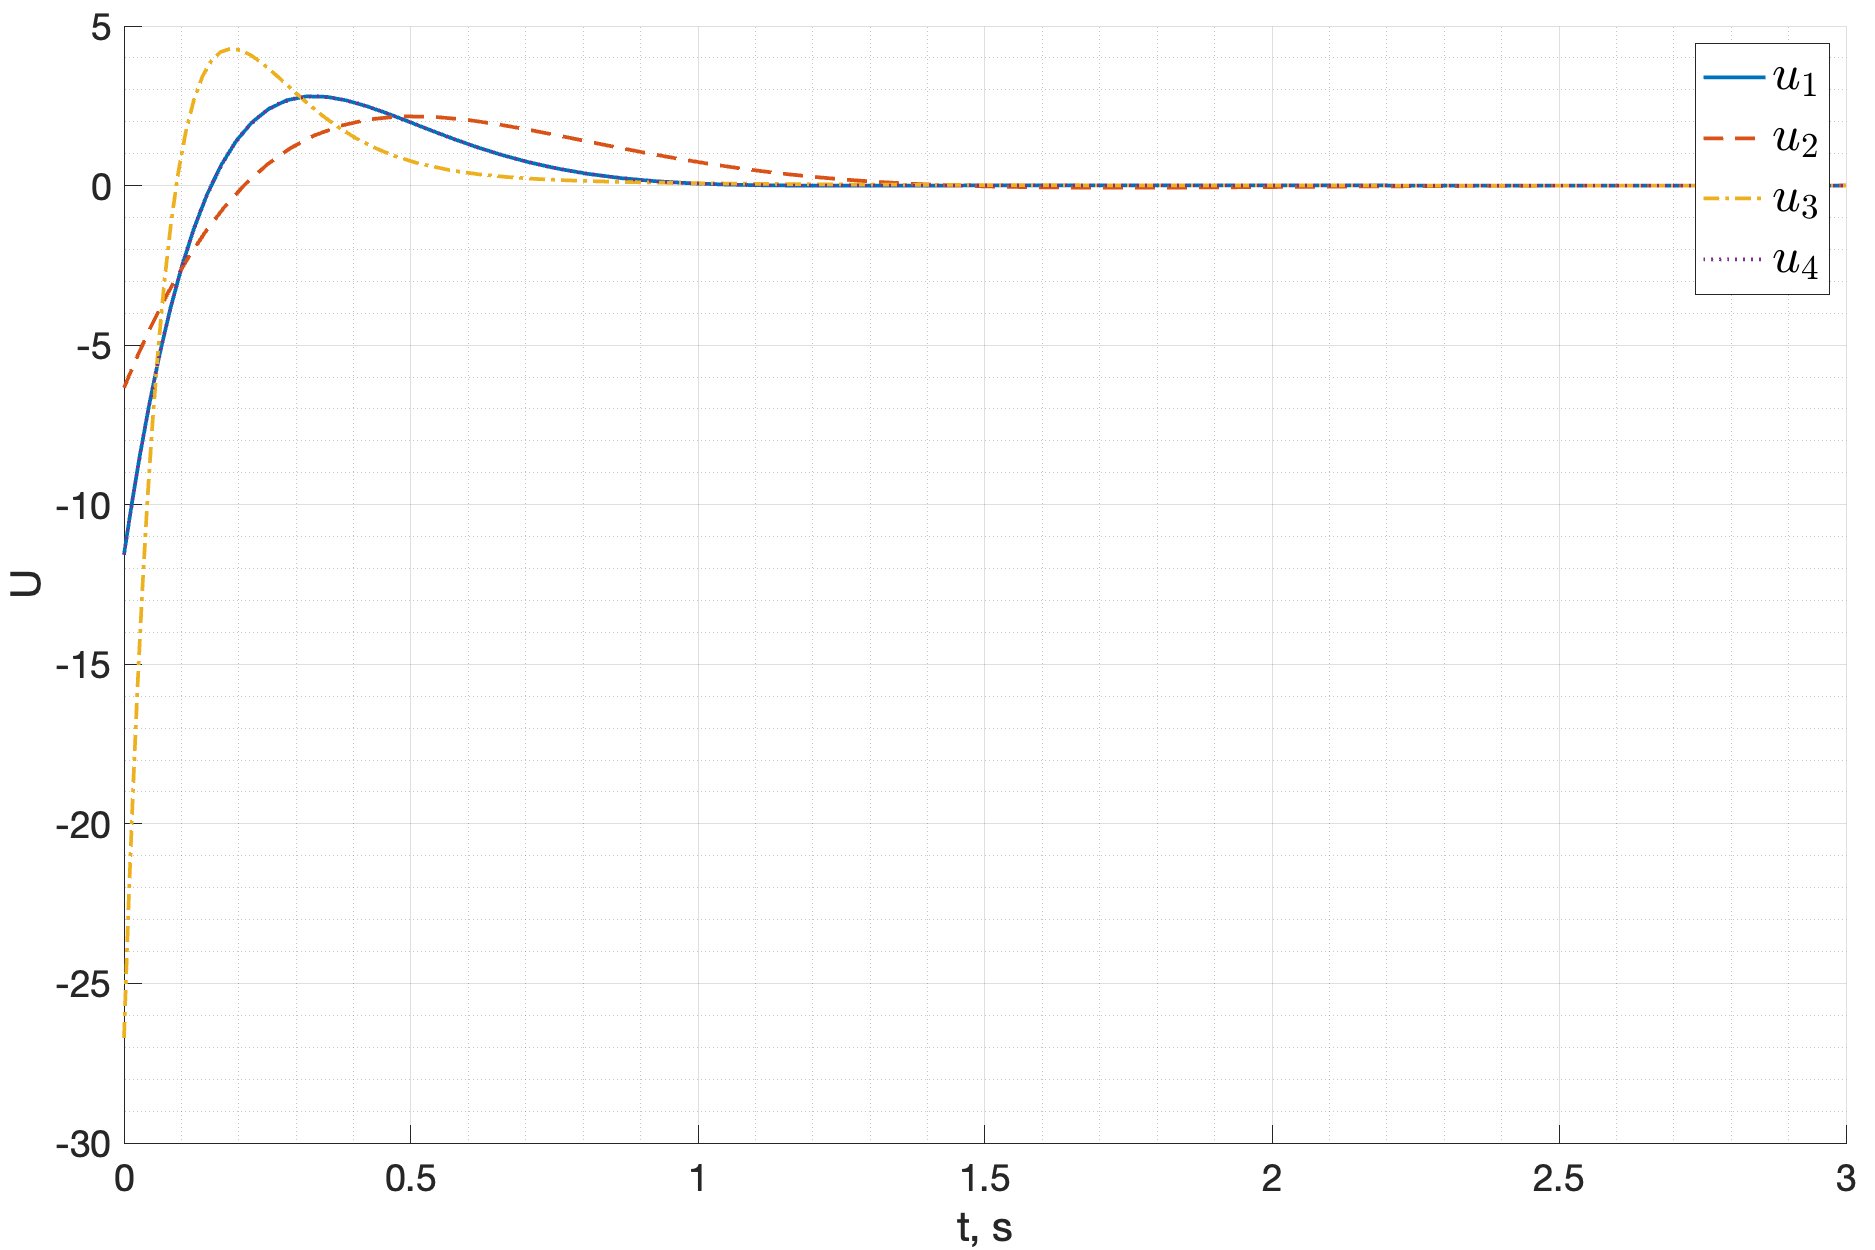
\includegraphics[width=\textwidth]{media/plots/lqr_task1/u_cmp.png}
    \caption{Управление системы с регуляторами $K_i$}
    \label{fig:task1_u}
\end{figure}
\begin{figure}[ht!]
    \centering
    \includegraphics[width=\textwidth]{media/plots/lqr_task1/j_cmp.png}
    \caption{Функционал качества $J$ для регуляторов $K_i$}
    \label{fig:task1_j}
\end{figure}
\begin{figure}[ht!]
    \centering
    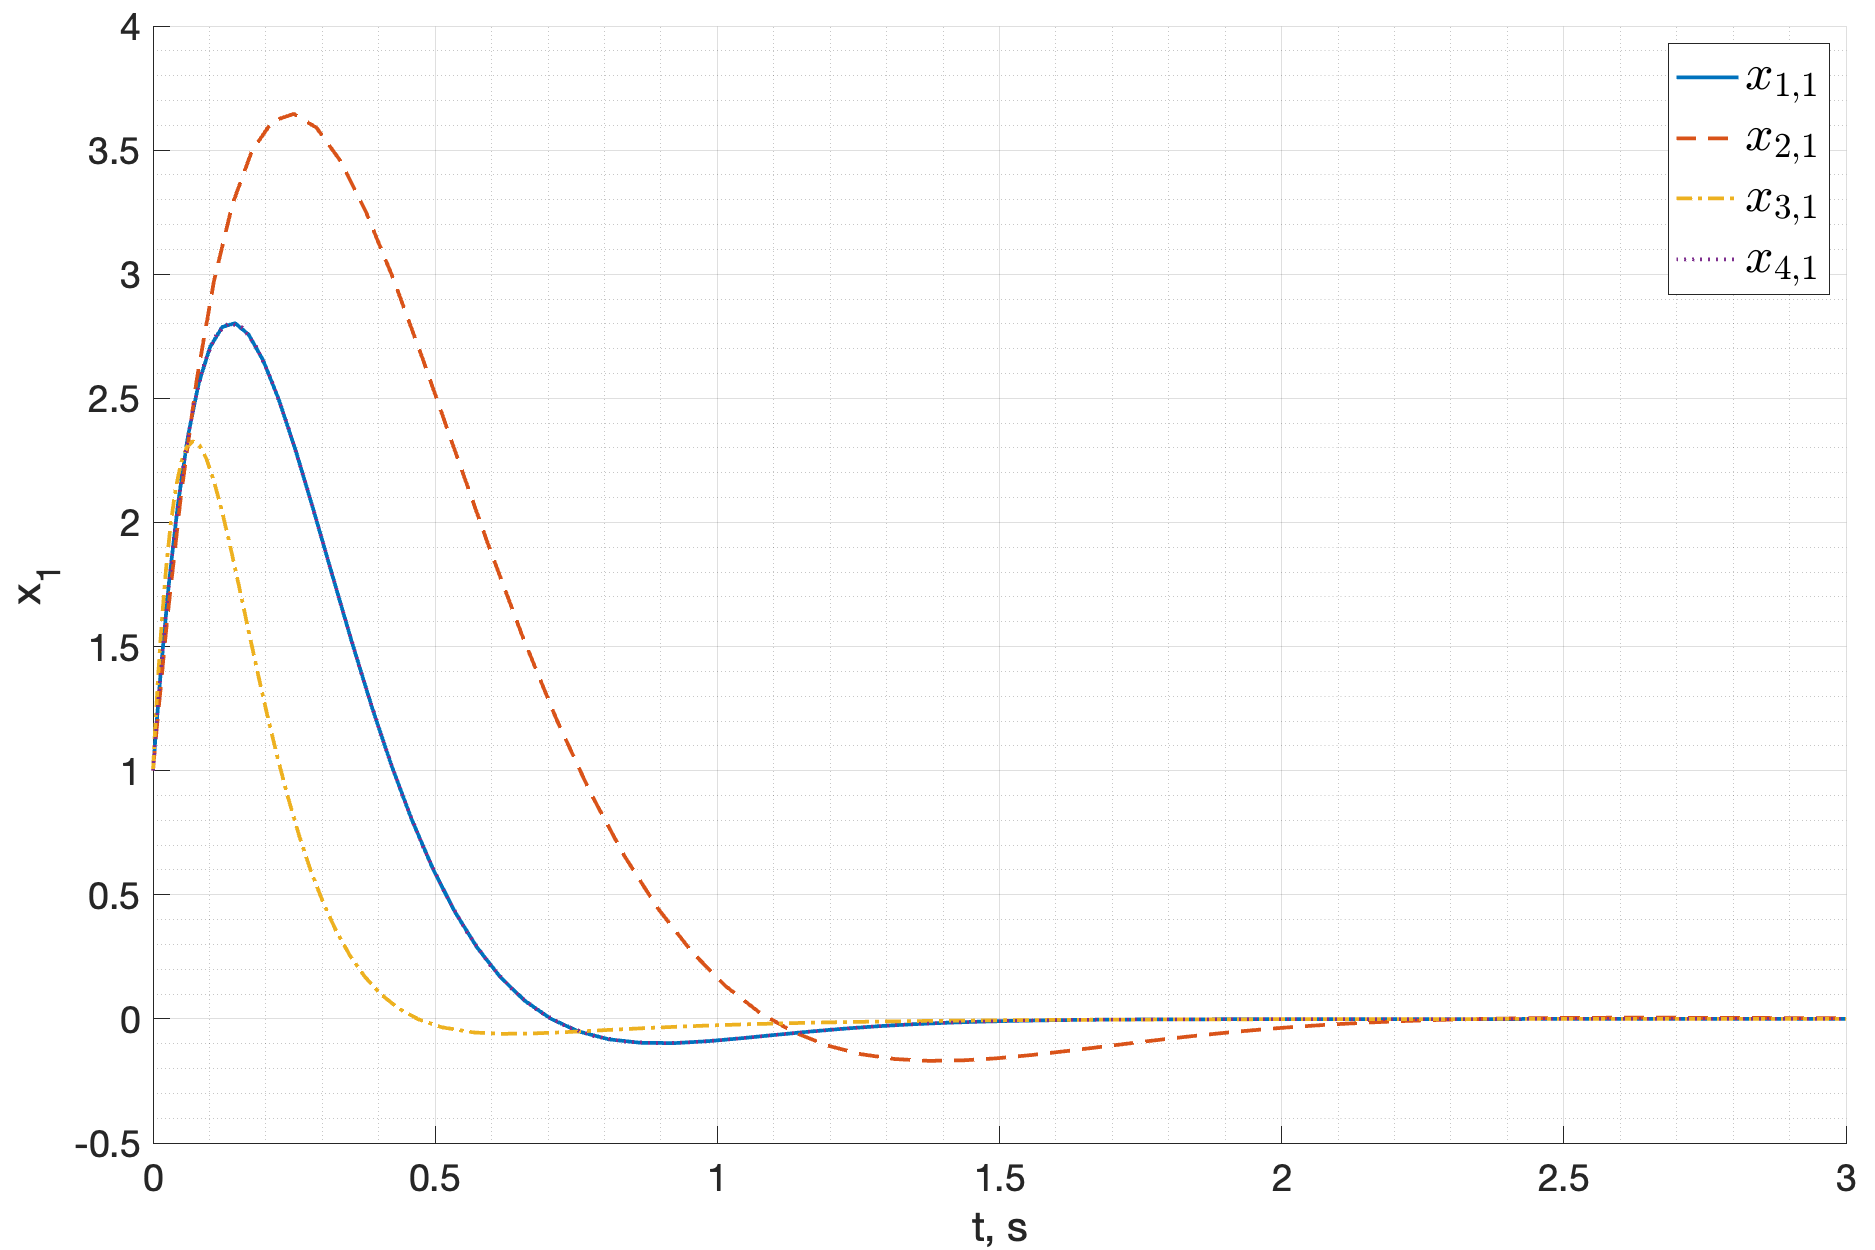
\includegraphics[width=\textwidth]{media/plots/lqr_task1/x1_cmp.png}
    \caption{Вектор состояние системы $x_1$}
    \label{fig:task1_x1_cmp_1}
\end{figure}
\begin{figure}[ht!]
    \centering
    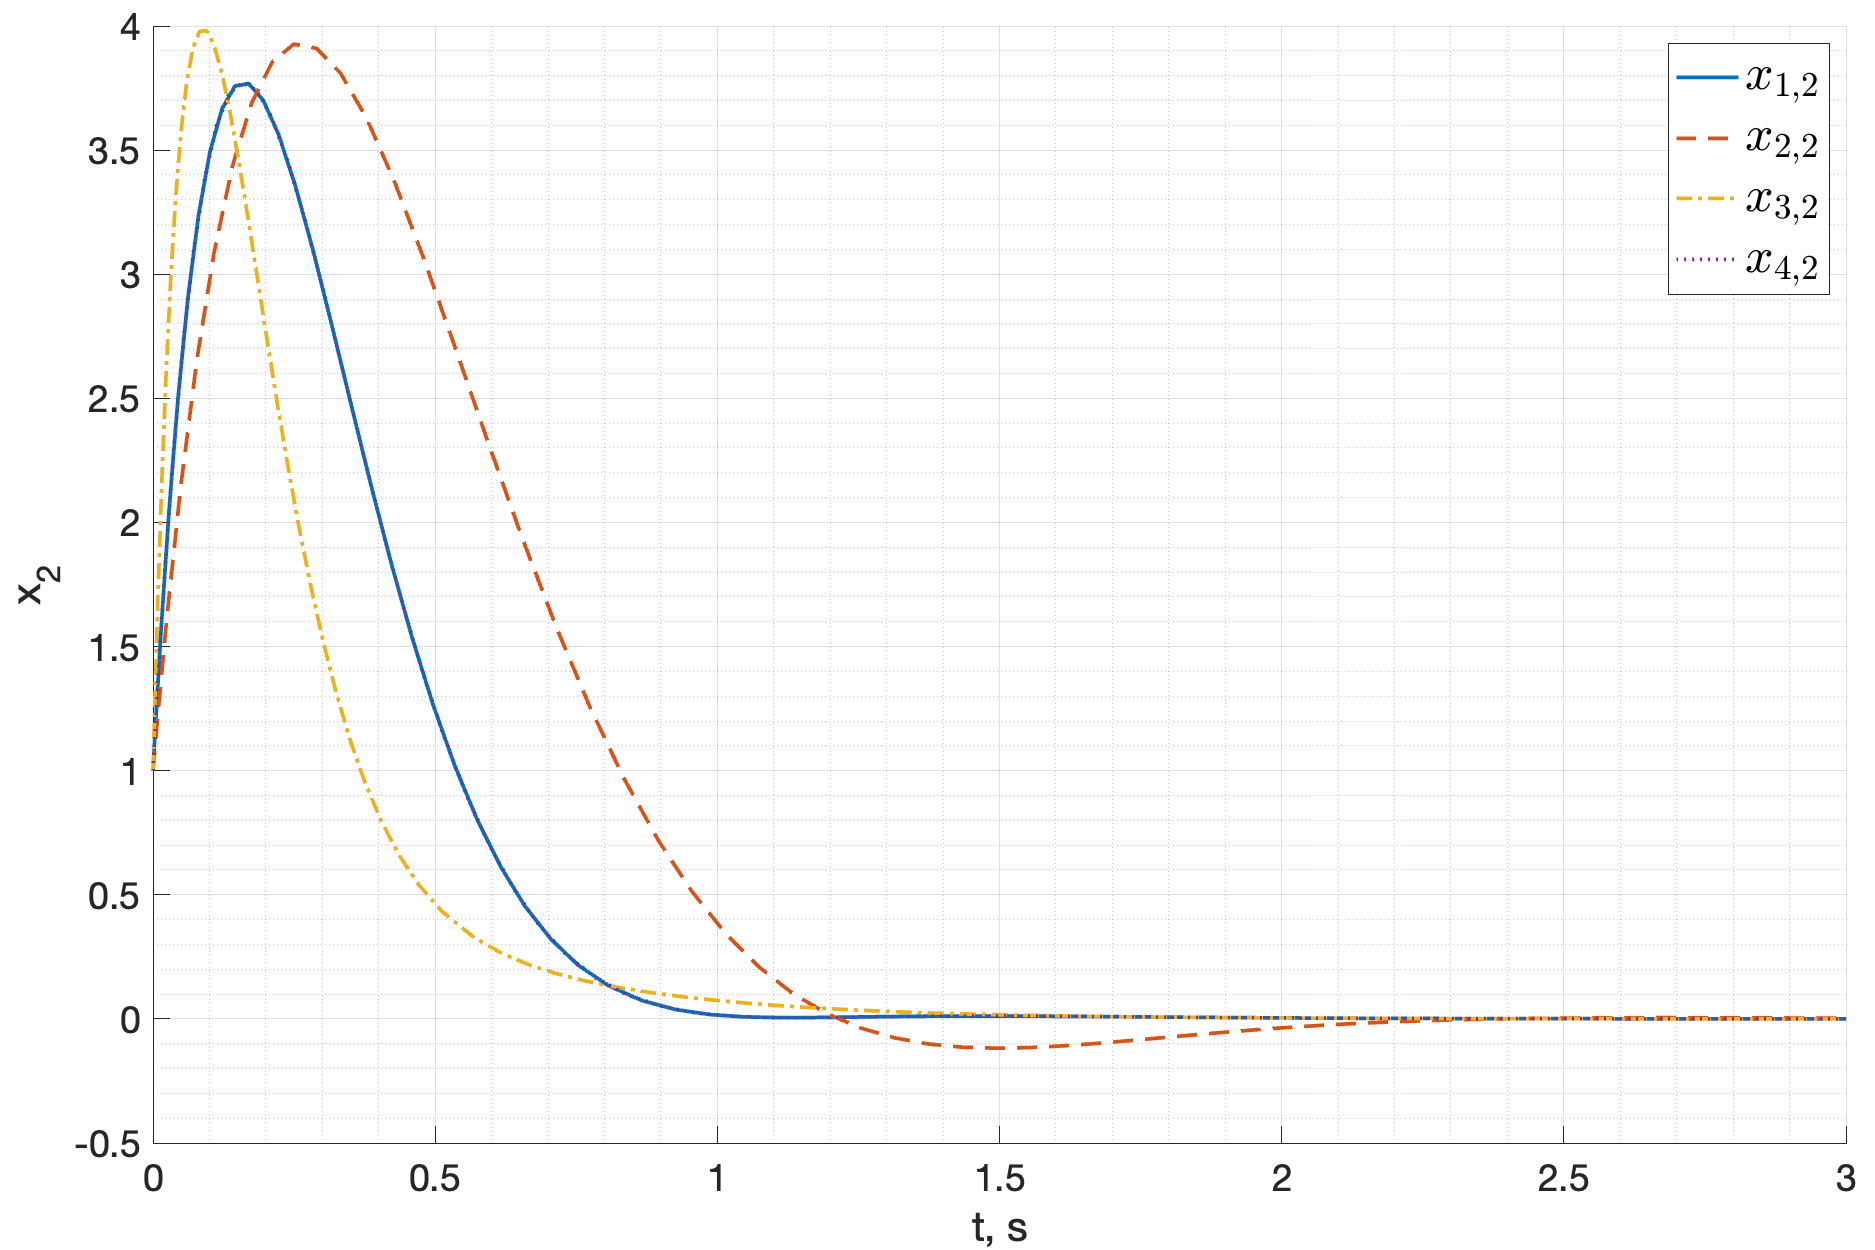
\includegraphics[width=\textwidth]{media/plots/lqr_task1/x2_cmp.png}
    \caption{Сравнение состояния системы $x_2$}
    \label{fig:task1_x2_cmp_1}
\end{figure}
\begin{figure}[ht!]
    \centering
    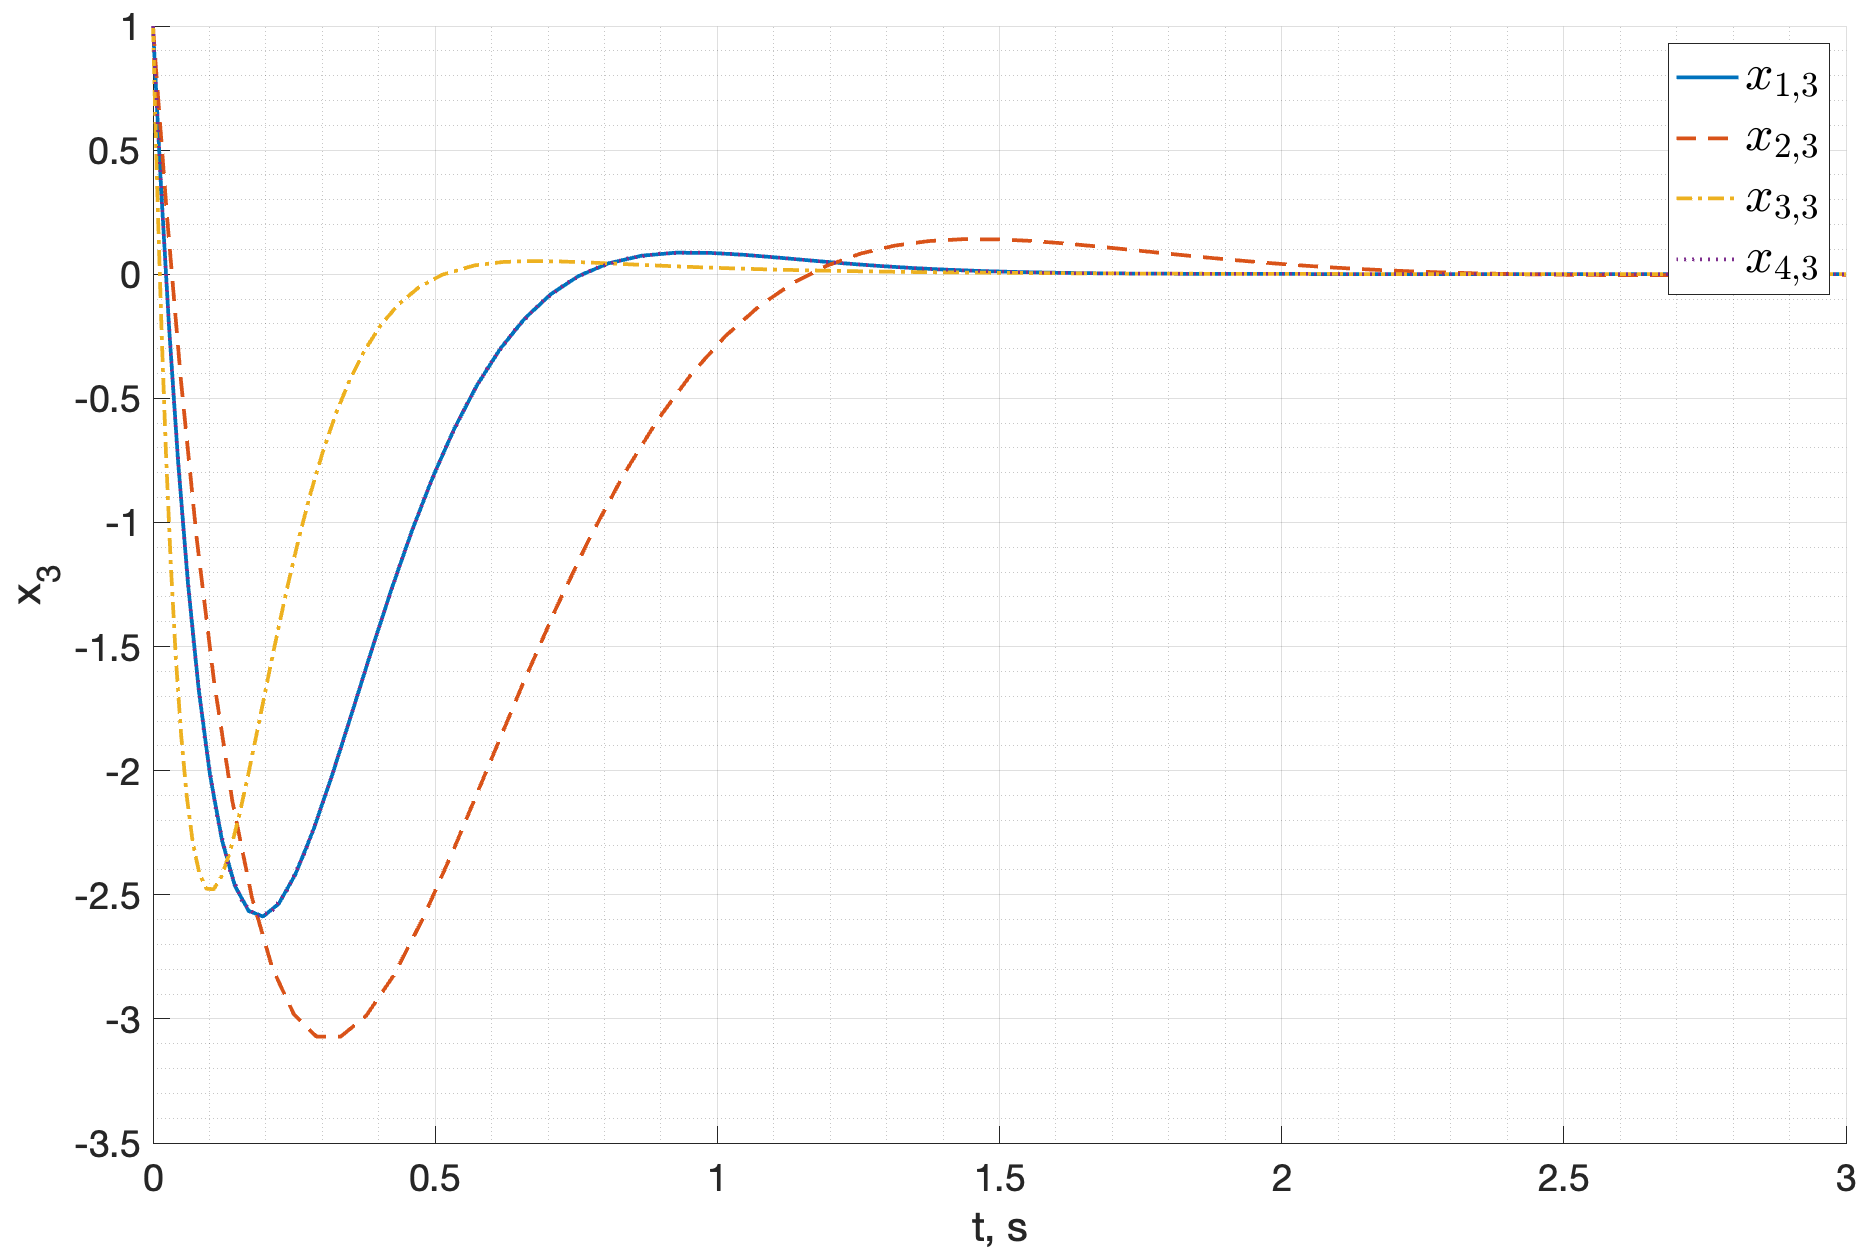
\includegraphics[width=\textwidth]{media/plots/lqr_task1/x3_cmp.png}
    \caption{Сравнение состояния системы $x_3$}
    \label{fig:task1_x3_cmp_1}
\end{figure}    
\FloatBarrier
\subsection{Выводы}
По данному исследования можно понять влияние матриц весов на поведение системы. 
Матрица $Q$ отвечает за штраф за отклонение состояния системы от желаемого значения, 
убедиться в этом можно сравнимая системы с регуляторами $K_1$ и $K_3$, $K_2$ и $K_4$. 
На рисунках \ref{fig:task1_x1_cmp_1} -- \ref{fig:task1_x3_cmp_1} хорошо видно, что при увеличении матрицы $Q$
компонентны вектора состояния системы $x$ стремятся к нулю быстрее, чем при меньшей матрицы $Q$. При этом, 
значения функционала качества $J$ для регуляторов $K_1$ и $K_1$ меньше, чем для $K_3$ и $K_4$, что 
говорит о том, что, при прочих равных, чем меньше матрица $Q$, тем меньше значение функционала качества, тем 
меньше энергии тратится на управление системой. 

Аналогично, матрица $R$ отвечает за штраф за использование \textit{резкого} управления. Тем больше значение 
матрицы $R$, тем тем более плавным становится управление системой, тем меньше перерегулирование, но при этом 
меньше скорость достижения нулевого состояния системы.  

Теоретические результаты вычисления минимизированного функционала качества $J_{min}$ для каждого регулятора $K_i$ совпадают с результатами моделирования, 
что видно на графике \ref{fig:task1_j}. 

Можно сделать вывод, что выбор матриц весов $Q$ и $R$ влияет на поведение системы, и получение желаемого поведения системы 
заключается в одновременном подборе матриц весов $Q$ и $R$. 